\chapter{The Cox Proportional Hazards Model \label{chapter:cox}}

We just encountered the Kaplan-Meier estimate of the survival function in Chapter~\ref{chapter:km}. Now we are going to talk about models that essentially treat the survival function as the \emph{outcome} in a supervised learning problem. These models are called \textbf{Cox proportional hazards models}.

%%%%%%%%%%%%%%%%%%%%%%%%%%%%%%%%%%%%%%%%%%%%%%%%%%%%%%%%%%%%%%%%%%%%%%%%%%%%%%%%%%

\section{Survival and Hazard Functions}

Consider a situation where we have some process that generates events, and we're trying to model the time to first event. Assume the probability of the event's occurring at each time, $t$, is given by the function $f(t)$. The cumulative probability of the event's having occurred by time $t$ is
$$ F(t) = \int_0^t f(t) dt$$
and the probability of an individual not having experienced the event by time $t$ is
$$ S(t) = 1 - F(t), $$
the \textbf{survival function}. The probability of experiencing the event in an infinitesimally small interval starting at $t$, given that one has not experienced it by time $t$, is:
$$ \lambda(t) = \frac{f(t)}{S(t)} $$
and is called the \textbf{hazard}. The \textbf{cumulative hazard} function is equal to
$$ \Lambda(t) = \int_0^t \lambda(t') dt' = -\log S(t) $$
so $S(t) = \exp(-\Lambda(t))$. 

None of these expressions should be immediately obvious to you, because deriving them requires calculus. It's a great exercise to go through the derivations, but for now, let's focus on capturing the intuition.

Here is a graphical representation of some of these quantities. Remember that the probability distribution $f(t)$ must integrate to one.

\begin{center}
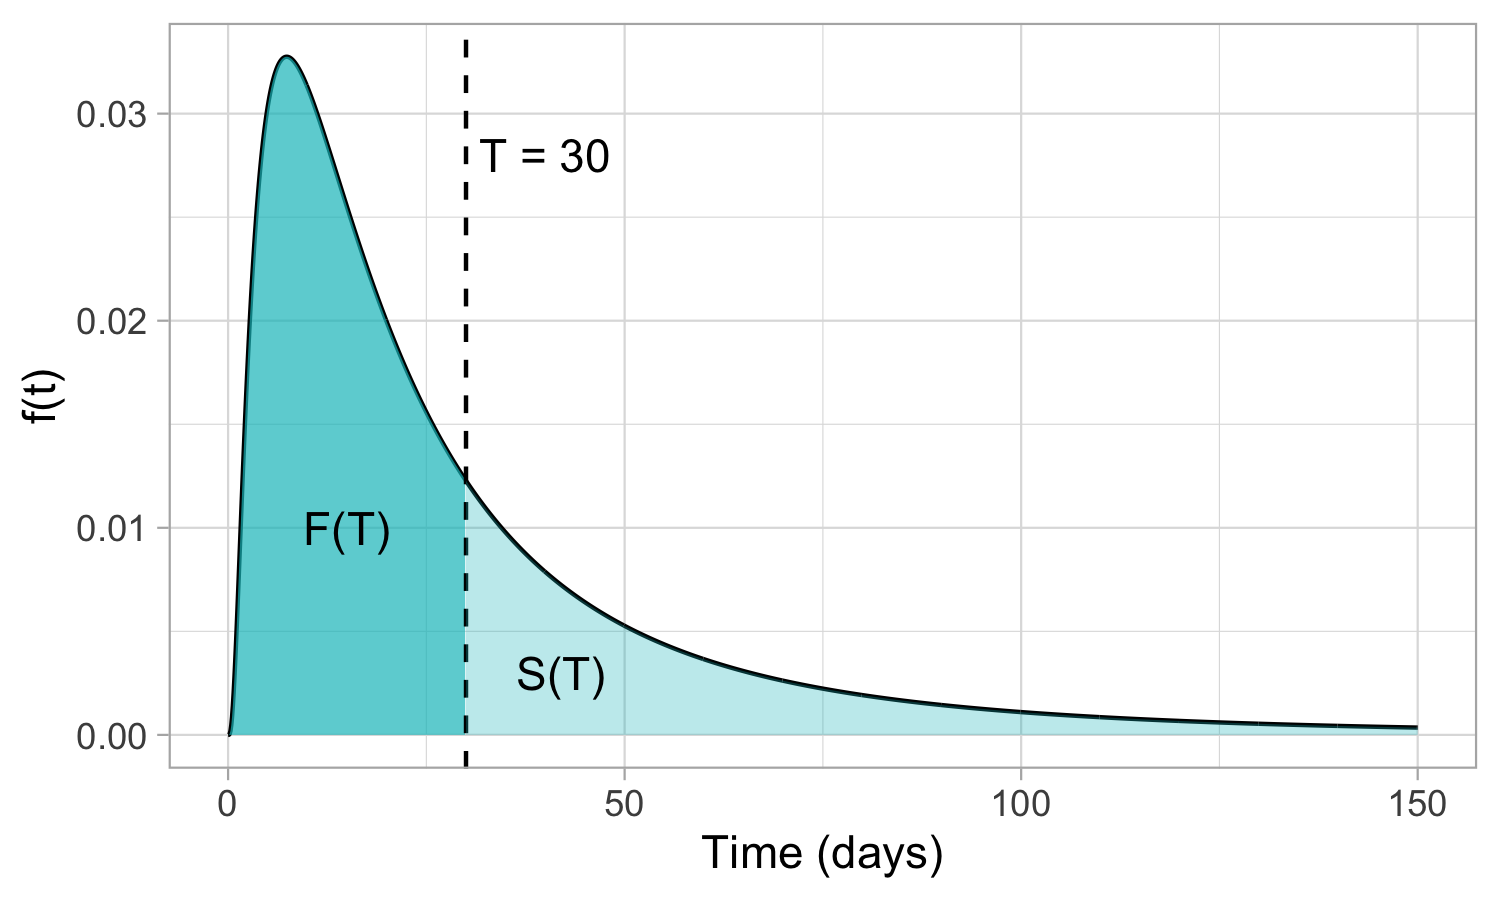
\includegraphics[width=0.85\textwidth]{img/survival-function-example-fx.png}
\end{center}

\vspace{3mm}

\begin{question}{}
What's the interpretation of the hazard, $\lambda(t)$, on this image? What happens to the hazard if $S(t)$ is low vs. high for the same $f(x)$? 
\end{question}

\begin{question}{}
Assume $f(t)$ is exponential: $f(t) = b \cdot \exp(-bt)$, where $b$ is constant. Then $F(t) = 1 - \exp(-bt)$ and $S(t) = \exp(-bt)$. What is the hazard, $\lambda(t)$? What is the cumulative hazard, $\Lambda(t)$? 
\end{question}

\vspace{3mm}

\begin{question}{}
The concept of a ``cumulative hazard'' is pretty weird. How should this quantity be interpreted?
% 1. The total amount of risk accumulated up to time t.
% 2. The number of times per subject that we would expect to observe failures over a given period if the failure event were repeatable.
% 3. It is useful in terms of allowing us to test assumptions of Cox models. Sort of like the logit in that way. It pops out of the modeling, so we care about it, but it isn't what we usually think about. 
\end{question}

%%%%%%%%%%%%%%%%%%%%%%%%%%%%%%%%%%%%%%%%%%%%%%%%%%%%%%%%%%%%%%%%%%%%%%%%%%%%%%%%%%

\section{Estimating Survival and Cumulative Hazard}

The Kaplan-Meier estimate of survival (Chapter~\ref{chapter:km}) is the most common estimate of the survival function. One can estimate the cumulative hazard using a couple of different methods. 
\begin{enumerate}
\item Take the negative log of the Kaplan-Meier estimate of survival:
\begin{align*} \hat{\Lambda}_{KM}(t) &= -\log \hat{S}_{\text{KM}}(t) \\
&= -\sum_{i:t_i < t} \log \left( 1 - \frac{d_i}{n_i} \right) \end{align*}
\item Use the \textbf{Nelson-Aalen estimator}
$$ \hat{\Lambda}_{NA}(t) = \sum_{i:t_i < t} \frac{d_i}{n_i} $$
\end{enumerate}

One thing that is confusing about the R \texttt{survival} package's output is that is uses the Kaplan-Meier estimate for survival by default, but it uses the Nelson-Aalen estimator for cumulative hazard by default. So if you exponentiate the negative cumulative hazard that comes out of \texttt{survfit}, it won't match the survival estimate. The two are close in most cases, though. Here are some pictures for the ovarian cancer survival dataset we discussed in Chapter~\ref{chapter:km}:

\begin{center}
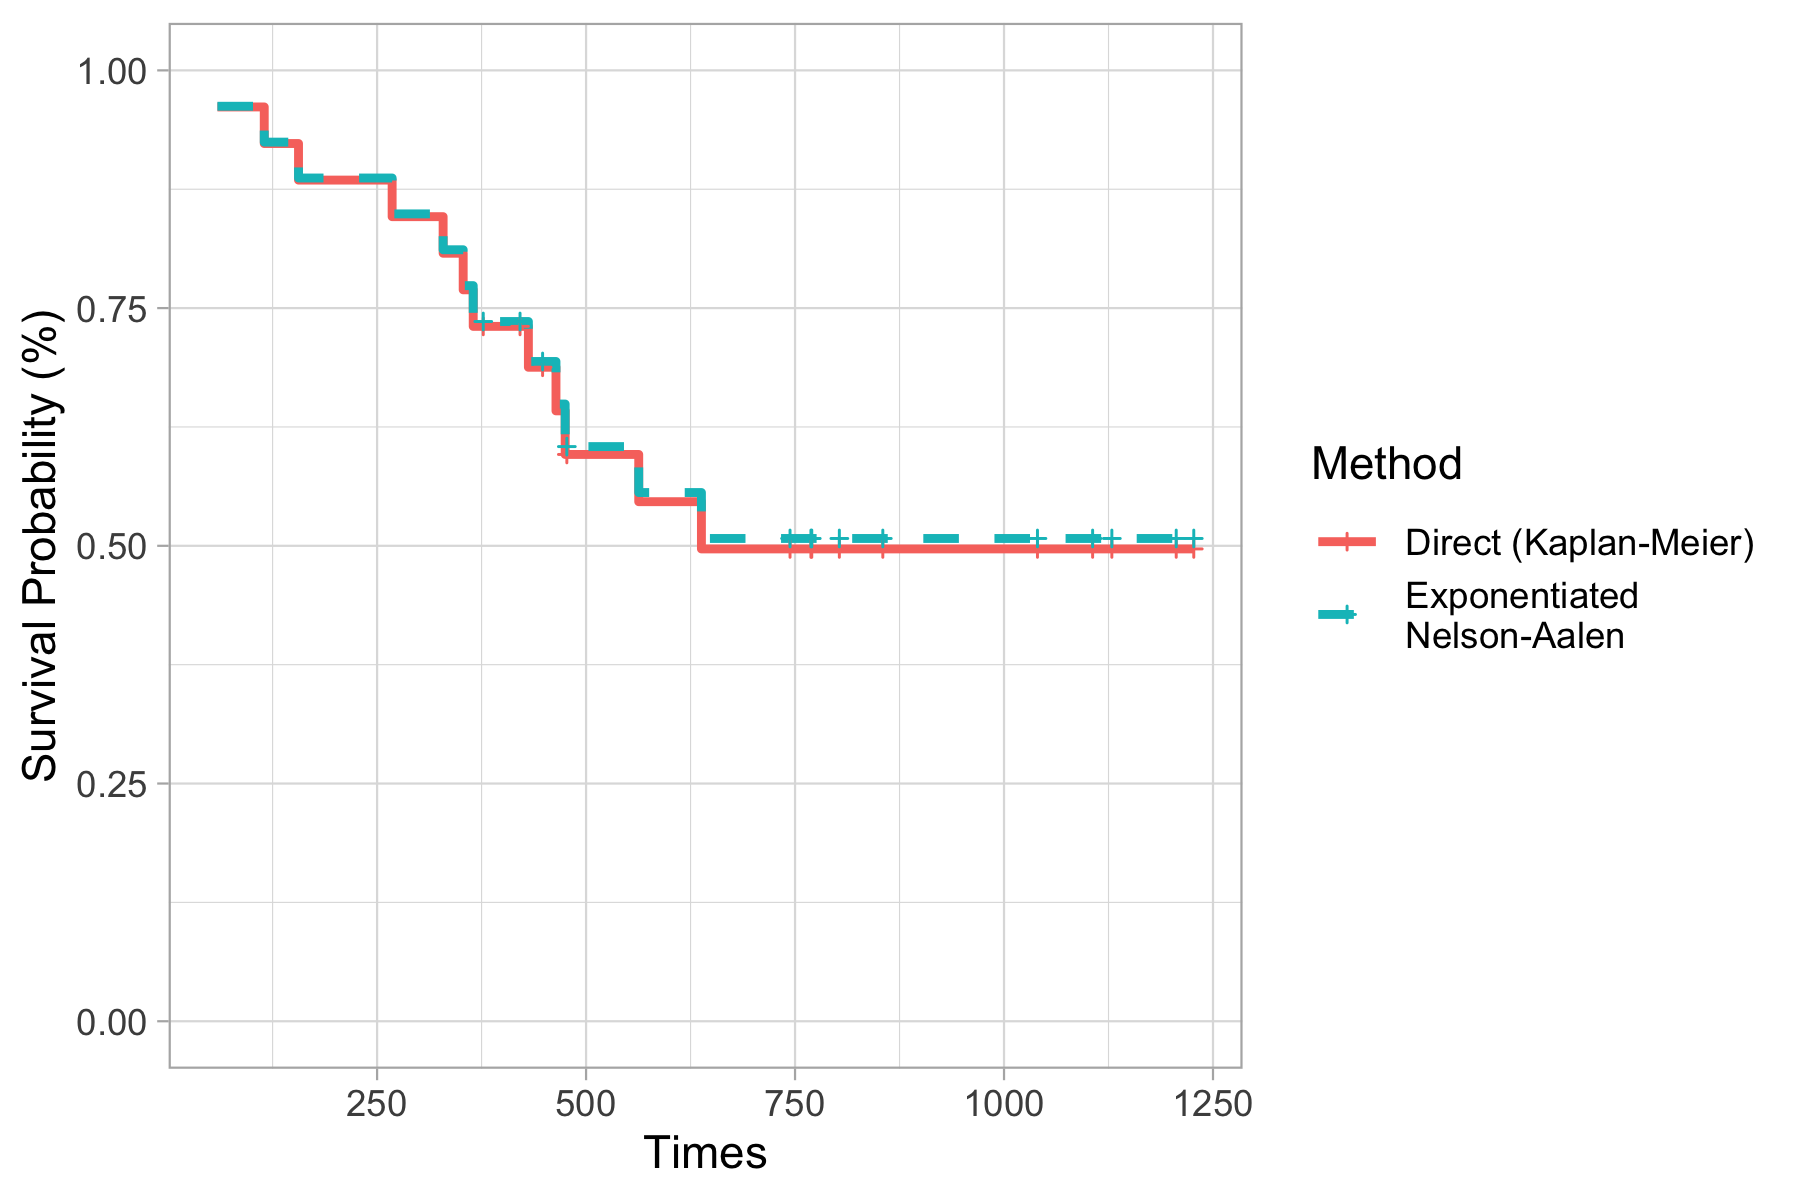
\includegraphics[width=0.85\textwidth]{img/ovarian-overall-survival.png}\\[3mm]
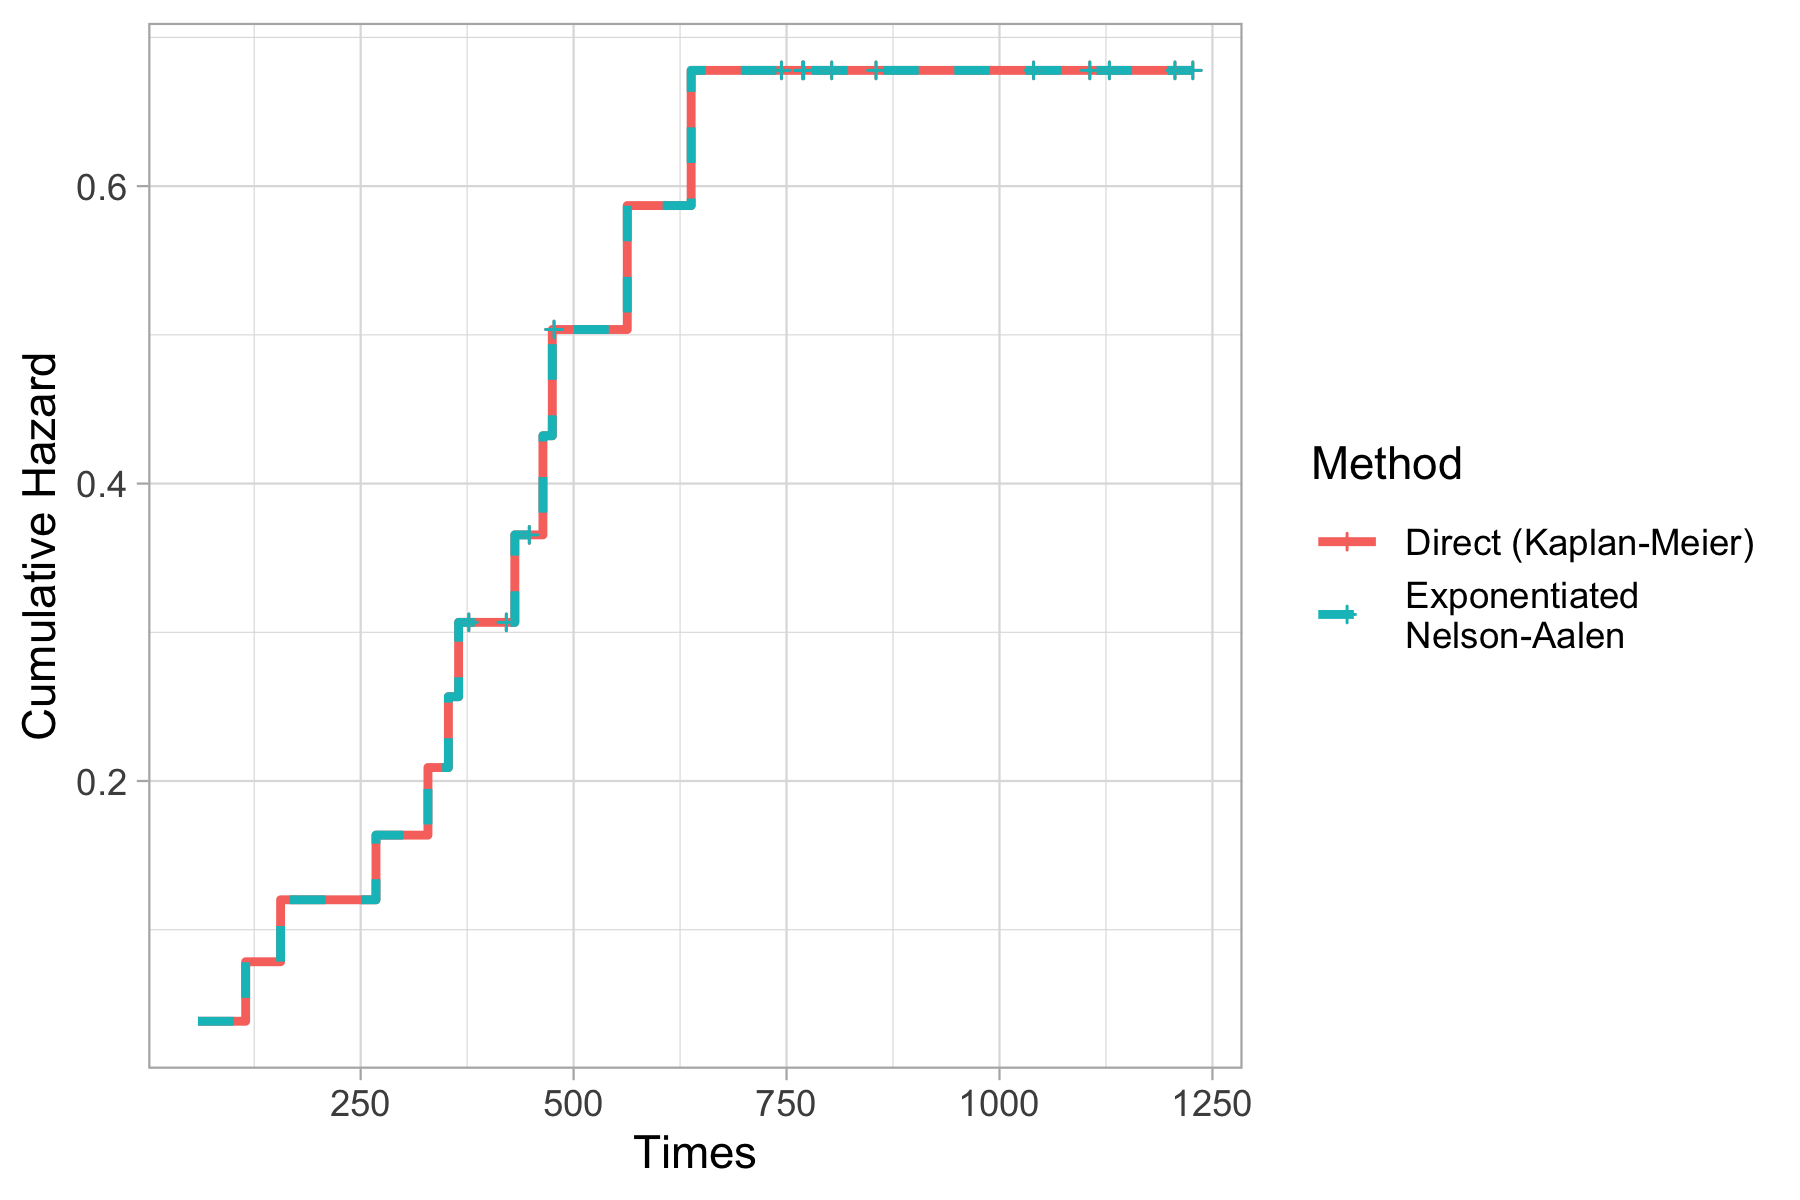
\includegraphics[width=0.85\textwidth]{img/ovarian-overall-cumhaz.png}
\end{center}

% From survfit.formula docs: "The routine returns both an estimated probability in state and an estimated cumulative hazard estimate. The cumulative hazard estimate is the Nelson-Aalen (NA) estimate or the Fleming-Harrington (FH) estimate, the latter includes a correction for tied event times. The estimated probability in state can estimated either using the exponential of the cumulative hazard, or as a direct estimate using the Aalen-Johansen approach. For single state data the AJ estimate reduces to the Kaplan-Meier and the probability in state to the survival curve; for competing risks data the AJ reduces to the cumulative incidence (CI) estimator. For backward compatability the type argument can be used instead."

\newpage

\begin{question}{}
Here is a plot showing the function $-\log(1-x)$ vs. $x$. Look at the expressions for the two estimators for the cumulative hazard, above. Under what conditions will they be similar? Under what conditions will they be different? 
\begin{center}
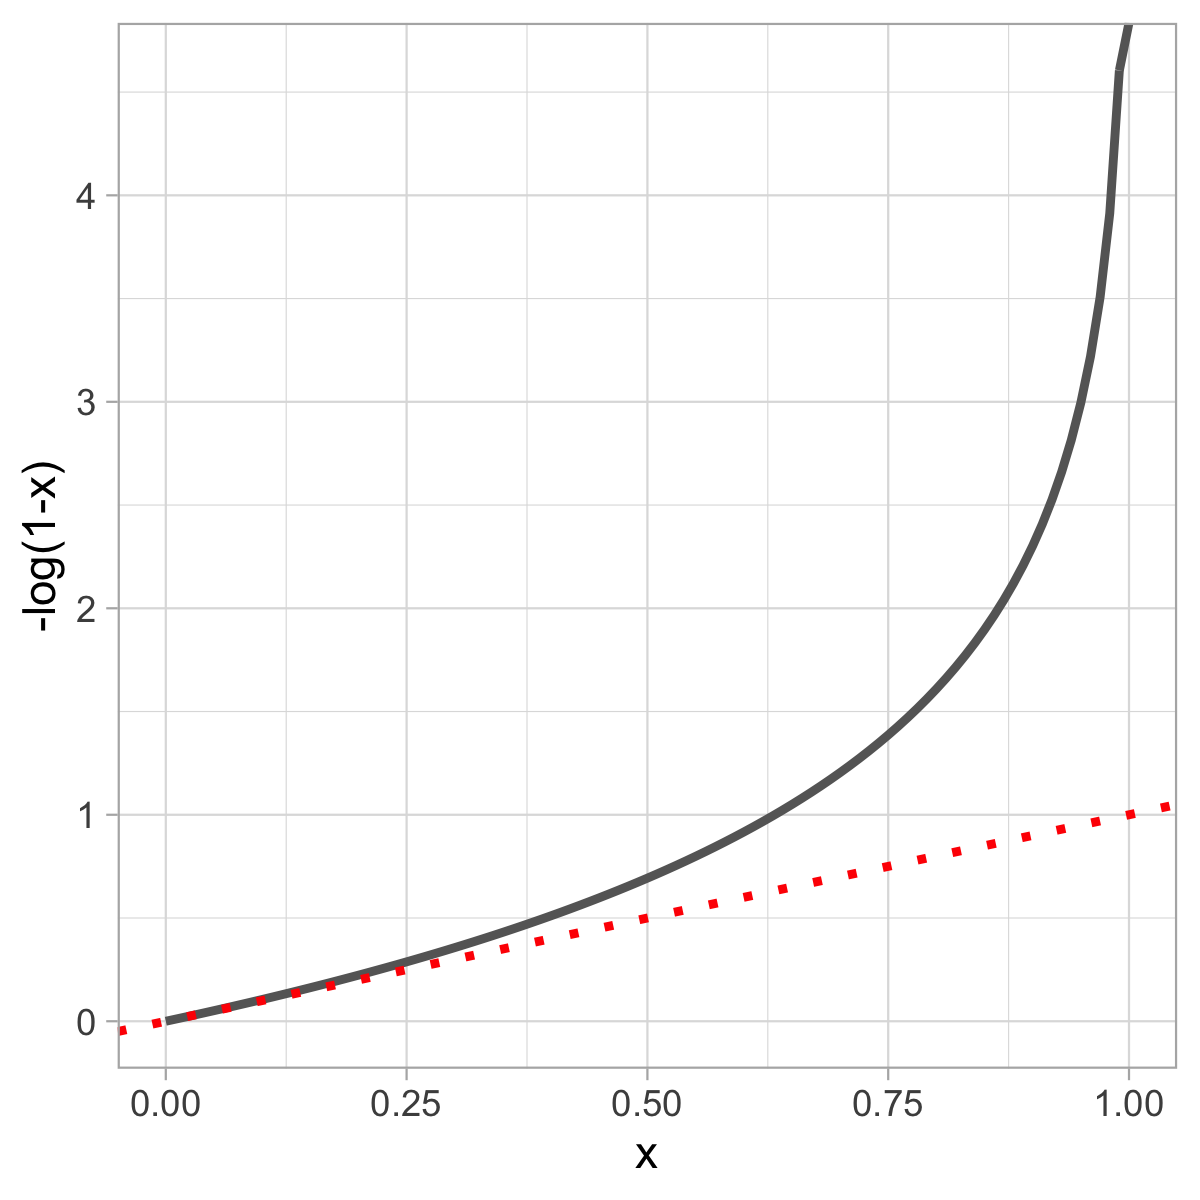
\includegraphics[width=0.6\textwidth]{img/survival-na-km-comparison.png}
\end{center} 
\end{question}

\vspace{3mm}

\begin{question}{}
The curvature of the Nelson-Aalen estimator gives you an idea of how the hazard varies with time. A concave shape is an indication of \emph{deceleration} of the hazard; for example, if the event in question is death and time is patient age, this would represent higher infant/childhood mortality than adult mortality. A convex shape is an indication of \emph{acceleration} of the hazard; in the death/age example, this would represent a process that accelerates as one ages (so called ``wear-out mortality''). 

Looking at the graph of the overall cumulative hazard, what do you notice about how the hazard for ovarian cancer changes since the initiation of treatment?
\end{question}

\newpage

\begin{question}{}
Here are the raw data from treatment group $1$ of the \texttt{ovarian} dataset. These are the same data we looked at when building the Kaplan-Meier curve in Chapter~\ref{chapter:km}, Question~\ref{question:kmo1}. Using these data, fill in the remaining cells of the table below. Here we are using the Nelson-Aalen estimator for the cumulative hazard. 
{\footnotesize
\begin{center}
\begin{tabular}{rlrr}
  \toprule
 & rx & futime & fustat \\ 
  \midrule
  1 & 1 & 59 & 1 \\ 
  2 & 1 & 115 & 1 \\ 
  3 & 1 & 156 & 1 \\ 
  4 & 1 & 268 & 1 \\ 
  5 & 1 & 329 & 1 \\ 
  6 & 1 & 431 & 1 \\ 
  7 & 1 & 448 & 0 \\ 
  8 & 1 & 477 & 0 \\ 
  9 & 1 & 638 & 1 \\ 
  10 & 1 & 803 & 0 \\ 
  11 & 1 & 855 & 0 \\ 
  12 & 1 & 1040 & 0 \\ 
  13 & 1 & 1106 & 0 \\ 
  \bottomrule
\end{tabular}
\end{center}
}
\vspace{-5mm}
{\footnotesize
\begin{center}
\begin{tabular}{rrrrll}
  \toprule
$j$ & $t_j$ & $n_j$ & $d_j$ & $\hat{\Lambda}(t_j)$ & Calculation \\ 
  \midrule
  0 & 0 & 13 & 0 & $0.000$ & $\frac{0}{13}$ \\
  1 & 59 & 13 & 1 & $0.077$ & $\hat{\Lambda}(t_0) + \frac{1}{13}$ \\
  2 & 115 & 12 & 1 & $0.160$ & $\hat{\Lambda}(t_1) + \frac{1}{12}$ \\[2mm]
  3 & 156 & \\[2mm] % 11 & 1 & $0.251$ & $\hat{\Lambda}(t_2) + \frac{1}{11}$ \\
  4 & 268 & \\[2mm] % 10 & 1 & $0.351$ & $\hat{\Lambda}(t_3) + \frac{1}{10}$ \\
  5 & 329 & 9 & 1 & $0.462$ & $\hat{\Lambda}(t_4) + \frac{1}{9}$ \\
  6 & 431 & 8 & 1 & $0.587$ & $\hat{\Lambda}(t_5) + \frac{1}{8}$ \\
  7 & 448 & 7 & 0 & $0.587$ & $\hat{\Lambda}(t_6) + \frac{0}{7}$ \\
  8 & 477 & 6 & 0 & $0.587$ & $\hat{\Lambda}(t_7) + \frac{0}{6}$ \\
  9 & 638 & 5 & 1 & $0.787$ & $\hat{\Lambda}(t_8) + \frac{1}{5}$ \\[2mm]
  10 & 803 & 4 & 0 & \\[2mm] % $0.787$ & $\hat{\Lambda}(t_9) + \frac{0}{4}$ \\
  11 & 855 & 3 & 0 & \\[2mm] % $0.787$ & $\hat{\Lambda}(t_{10}) + \frac{0}{3}$ \\
  12 & 1040 & 2 & 0 & \\[2mm] % $0.787$ & $\hat{\Lambda}(t_{11}) + \frac{0}{2}$ \\
  13 & 1106 & 1 & 0 & \\[2mm] % $0.787$ & $\hat{\Lambda}(t_{12}) + \frac{0}{1}$ \\
  \bottomrule
\end{tabular}
\end{center}
}
\end{question}

\newpage

\begin{question}{}
Here are plots of the cumulative hazard (Nelson-Aalen estimator) for patients by sex and by ECOG performance score status:
\begin{center}
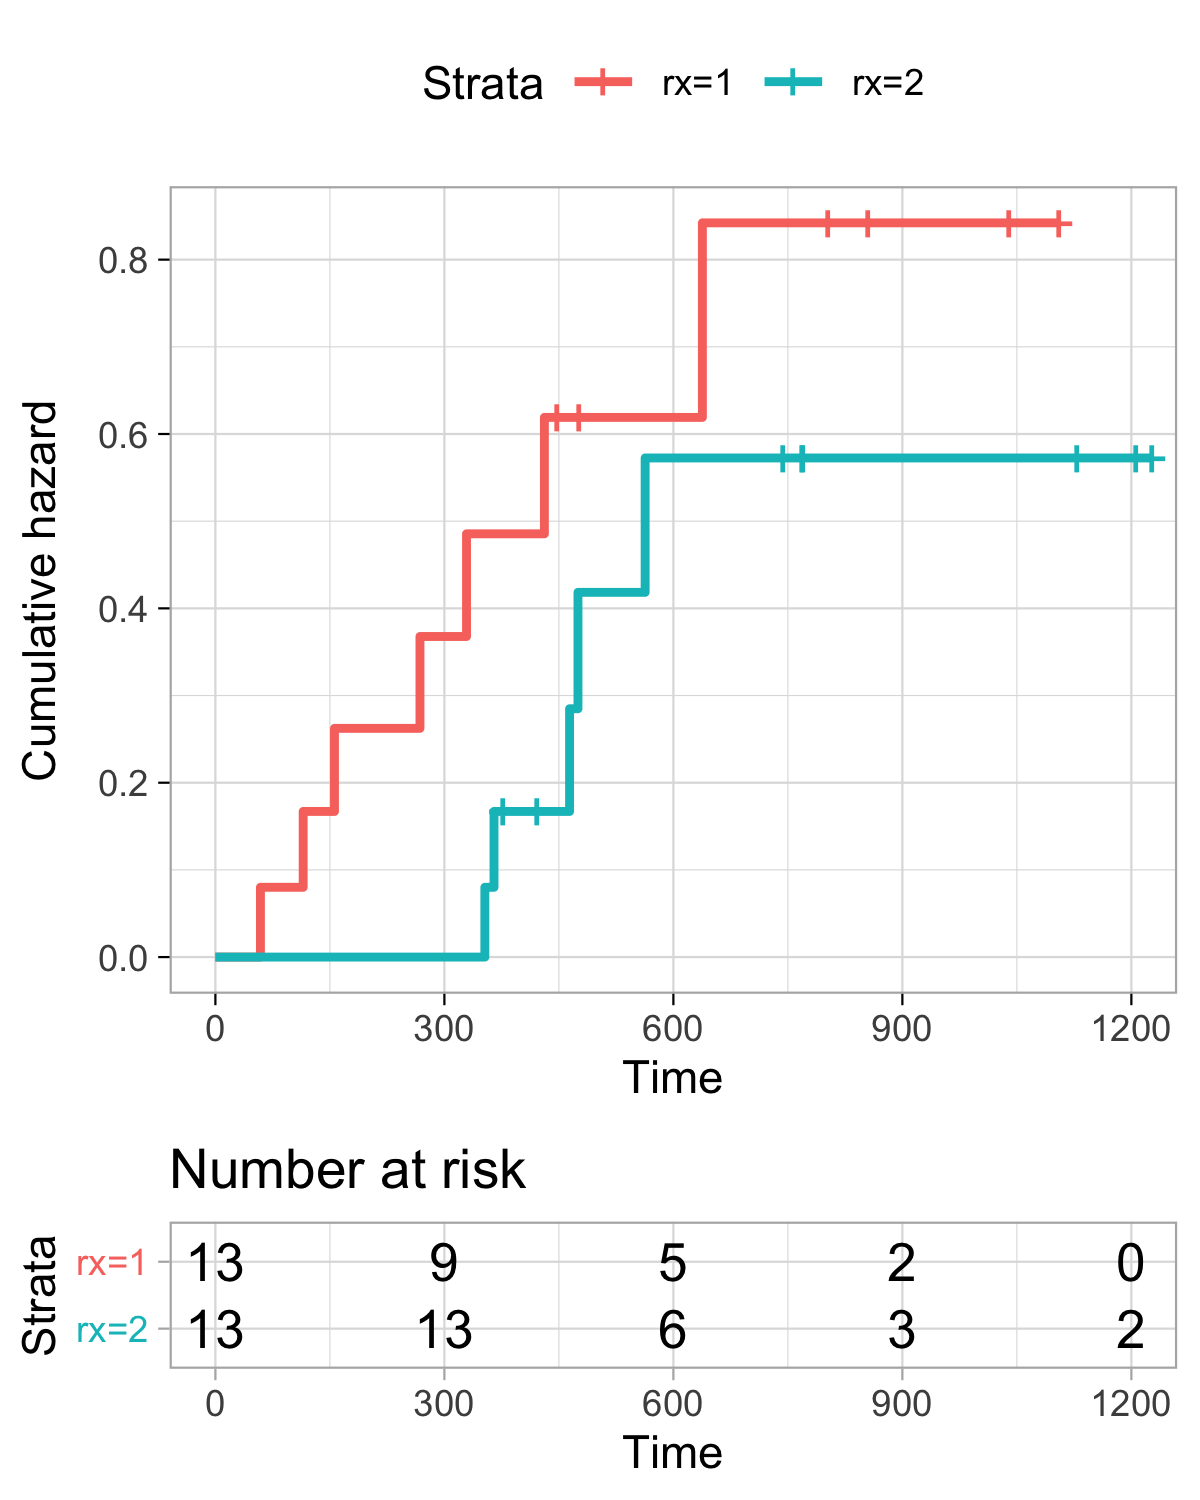
\includegraphics[width=0.45\textwidth]{img/ovarian-rx-cumhaz.png}
\hspace{4mm}
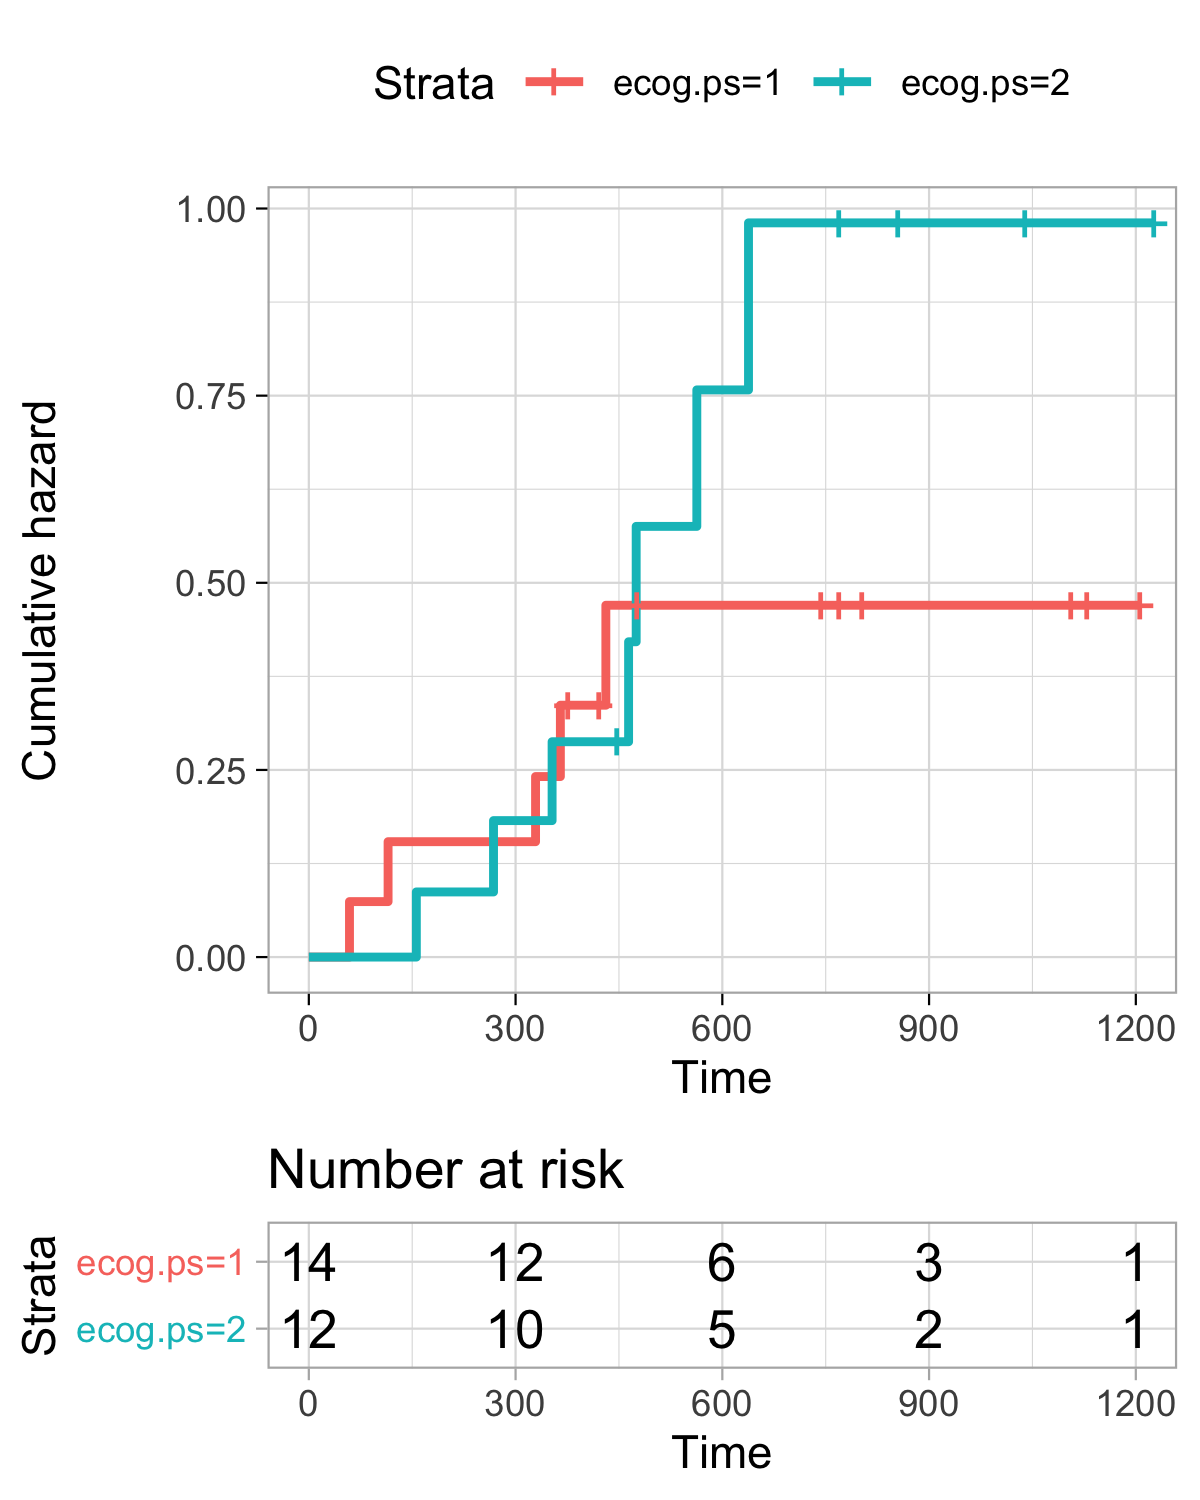
\includegraphics[width=0.45\textwidth]{img/ovarian-ecog-cumhaz.png}
\end{center}
How does treatment group appear to impact the cumulative hazard? What about ECOG score? Do the cumulative hazards appear proportional (i.e., related by a common multiplier) in each case? 
\end{question}

%%%%%%%%%%%%%%%%%%%%%%%%%%%%%%%%%%%%%%%%%%%%%%%%%%%%%%%%%%%%%%%%%%%%%%%%%%%%%%%%%%

\section{Deriving the Cox Model}

We have spent considerable time on the hazard and cumulative hazard because these play important roles in what is perhaps the most famous survival analysis tool: the Cox proportional hazards model (``Cox model'', for short), developed by D.R. Cox in 1972. The model has the following form:
$$ \lambda(t|x) = \lambda_0(t)\exp(\beta_1 x_1 + \beta_2 x_2 + \dots + \beta_p x_p) $$
and another way of writing it is:
$$ \log \left( \frac{\lambda(t|x)}{\lambda_0(t)} \right) = \beta_1 x_1 + \beta_2 x_2 + \dots + \beta_p x_p. $$
Note that for now we are assuming that the covariates do not depend on time. There is a variant of the Cox model called the \textbf{extended Cox model} that allows time-dependent covariates. For now, we will just consider the fixed covariate case. 

\vspace{3mm}

\begin{question}{}
Compare the Cox model to a logistic regression model. What is the same? What is different?
\end{question}

Here $\lambda_0(t)$ is called the \textbf{baseline hazard}. As usual, we symbolize the linear sum of the $\beta$s as $\beta^Tx$. Importantly, the baseline hazard can take any shape as a function of time. The $\lambda_0(t)$ part of the equation is, therefore, referred to as the ``nonparametric'' part, while the $\beta^Tx$ part is called the ``parametric'' part. The overall model is referred to as \textbf{semiparametric}. 

The ratio of the hazards for two different sets of covariates, $x$ and $z$, is
$$ \frac{\lambda(t|x)}{\lambda(t|z)} = \frac{\lambda_0(t)\exp(\beta^Tx)}{\lambda_0(t)\exp(\beta^Tz)} = \exp(\beta^T (x-z)). $$
Taking the log of this, we arrive at
$$ \log \left( \frac{\lambda(t|x)}{\lambda(t|z)} \right) = \beta^T (x-z). $$
A single coefficient, $\beta_j$, is therefore the \textbf{hazard ratio} when the corresponding predictor, $x_j$, increases by one. This ratio is assumed to be constant over time. The hazard ratio is also called the \textbf{relative risk}. 

\vspace{5mm}

\begin{question}{}
Why doesn't the Cox model have an intercept, $\beta_0$?
\end{question}

\vspace{1mm}

\begin{question}{}
Compare the interpretation of the coefficients in a Cox model to their interpretation in a logistic regression model. 
\end{question}

%%%%%%%%%%%%%%%%%%%%%%%%%%%%%%%%%%%%%%%%%%%%%%%%%%%%%%%%%%%%%%%%%%%%%%%%%%%%%%%%%%

\section{Fitting the Cox Model \label{section:coxfit}}

Fitting a Cox model means taking a sample of possibly right-censored data and deriving estimates for the parameters, $\beta_1, \dots, \beta_p$. Cox models are fit using a variant of maximum likelihood estimation called \textbf{partial likelihood estimation}.

Let's consider all of the unique times, $t_i$, that events are observed. For now, we will assume that exactly one event is observed at each of these times (no ties). We will use $R(t_i)$ to refer to the set of subjects who are ``at risk'' (i.e., not censored) just prior to time $t_i$. At each failure time, $t_i$, the contribution to the partial likelihood is:
\begin{align*} \mathcal{L}_i(\beta) &= \frac{P(\text{person $i$ experiences event|still around at $t_i$)}}{\sum_{l \in R(t_i)} P(\text{person $l$ experiences event|still around at $t_i$)}} \\
&= \frac{\lambda(t_i|x_i)}{\sum_{l \in R(t_i)} \lambda(t_i|x_l)} = \frac{\exp(\beta^Tx^{(i)})}{\sum_{l \in R(t_i)} \exp( \beta^Tx^{(l)})} \end{align*} 
The complete partial likelihood over all $K$ observed event times, $t_i = t_1, \dots, t_K$, is:
$$ \mathcal{L}(\beta) = \prod_{i=1}^K \frac{\exp(\beta^Tx^{(i)})}{\sum_{l \in R(t_i)} \exp( \beta^Tx^{(l)})}.  $$
This is the thing that the model fitting process is trying to maximize. It is optimized numerically, using the same types of optimization procedures used by logistic regression and other generalized linear models.

\vspace{3mm}

\begin{question}{}
Why is this quantity called a ``partial likelihood'', instead of just a ``likelihood''?
\end{question} 

%%%%%%%%%%%%%%%%%%%%%%%%%%%%%%%%%%%%%%%%%%%%%%%%%%%%%%%%%%%%%%%%%%%%%%%%%%%%%%%%%%

\section{Interpreting Cox Models}

Here is a simple Cox model for survival time vs. age, residual disease, ECOG score, and treatment group in the ovarian cancer dataset.

\begin{center}
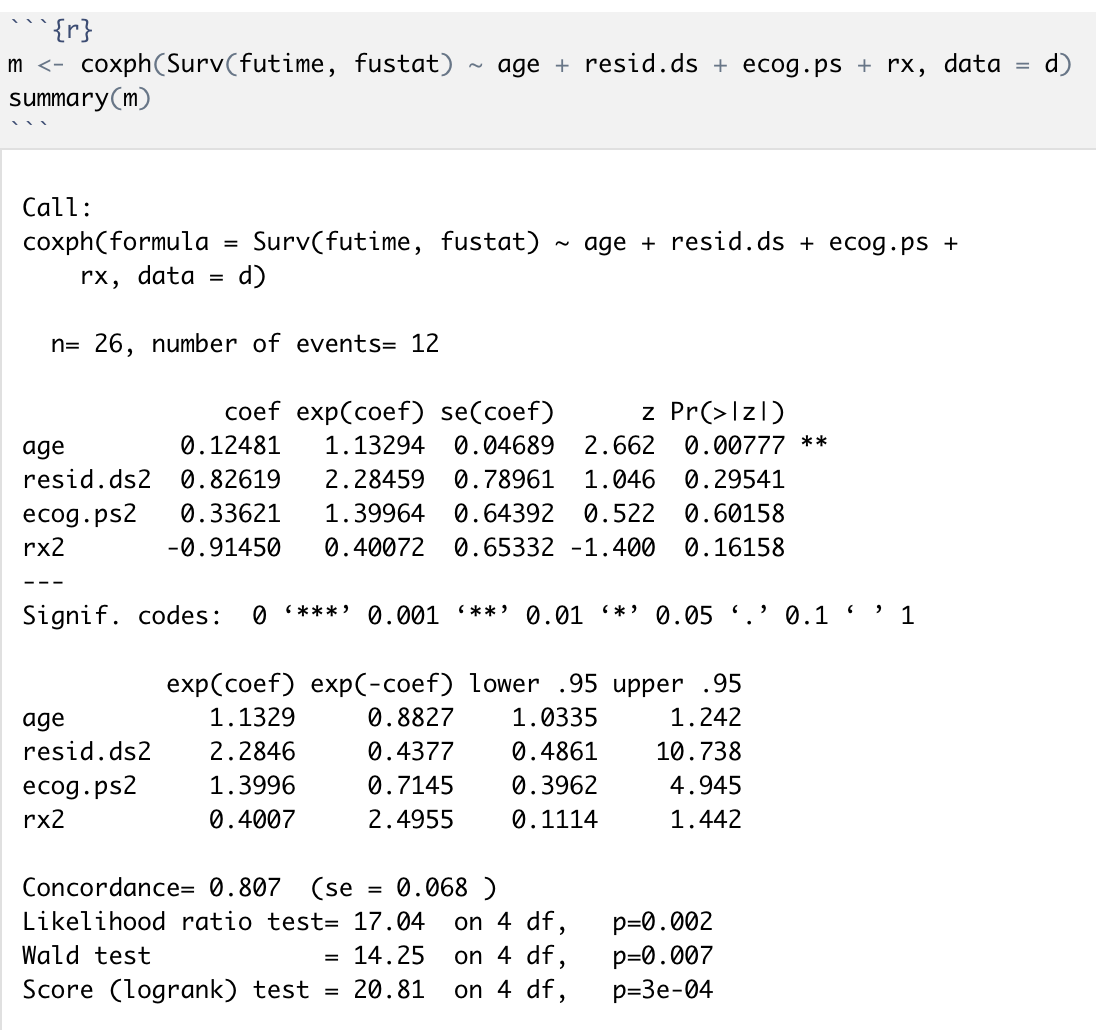
\includegraphics[width=0.9\textwidth]{img/ovarian-coxph-model.png}
\end{center}

\vspace{3mm}

\begin{question}{}
Interpret the coefficients, exponentiated coefficients, standard errors of the coefficients, Z scores, and $p$-values in this model. Also try your hand at interpreting the second block of model output, which includes the exponentiated coefficients (again), the exponentiated negative coefficients, and the lower and upper bounds of a 95\% confidence interval for the exponentiated coefficients.
\end{question}

%%%%%%%%%%%%%%%%%%%%%%%%%%%%%%%%%%%%%%%%%%%%%%%%%%%%%%%%%%%%%%%%%%%%%%%%%%%%%%%%%%

\section{Making Predictions with Cox Models}

The Cox model fitted using the \texttt{coxph} function can be used to make various predictions on the original dataset. This yields a lot of output. All of the available outputs for the \texttt{ovarian} dataset are shown below. 

{\scriptsize
\begin{center}
\begin{tabular}{rrrrrrrrrrrrr}
  \toprule
 & age & lp\_age & resid.ds & lp\_resid.ds & ecog.ps & lp\_ecog.ps & rx & lp\_rx & lp & risk & expected & surv \\ 
  \midrule
  1 & 72.33 & 9.03 & 2 & 0.83 & 1 & 0.00 & 1 & 0.00 & 2.67 & 14.43 & 0.16 & 0.85 \\ 
  2 & 74.49 & 9.30 & 2 & 0.83 & 1 & 0.00 & 1 & 0.00 & 2.94 & 18.90 & 0.46 & 0.63 \\ 
  3 & 66.47 & 8.30 & 2 & 0.83 & 2 & 0.34 & 1 & 0.00 & 2.27 & 9.71 & 0.40 & 0.67 \\ 
  4 & 53.36 & 6.66 & 2 & 0.83 & 1 & 0.00 & 2 & -0.91 & -0.61 & 0.54 & 0.11 & 0.89 \\ 
  5 & 50.34 & 6.28 & 2 & 0.83 & 1 & 0.00 & 1 & 0.00 & -0.08 & 0.93 & 0.25 & 0.78 \\ 
  6 & 56.43 & 7.04 & 1 & 0.00 & 2 & 0.34 & 1 & 0.00 & 0.19 & 1.21 & 0.33 & 0.72 \\ 
  7 & 56.94 & 7.11 & 2 & 0.83 & 2 & 0.34 & 2 & -0.91 & 0.17 & 1.18 & 0.40 & 0.67 \\ 
  8 & 59.85 & 7.47 & 2 & 0.83 & 2 & 0.34 & 2 & -0.91 & 0.53 & 1.71 & 0.70 & 0.49 \\ 
  9 & 64.18 & 8.01 & 2 & 0.83 & 1 & 0.00 & 1 & 0.00 & 1.65 & 5.21 & 2.15 & 0.12 \\ 
  10 & 55.18 & 6.89 & 1 & 0.00 & 2 & 0.34 & 2 & -0.91 & -0.88 & 0.42 & 0.24 & 0.79 \\ 
  11 & 56.76 & 7.08 & 1 & 0.00 & 2 & 0.34 & 1 & 0.00 & 0.24 & 1.27 & 0.94 & 0.39 \\ 
  12 & 50.11 & 6.25 & 1 & 0.00 & 1 & 0.00 & 2 & -0.91 & -1.84 & 0.16 & 0.12 & 0.89 \\ 
  13 & 59.63 & 7.44 & 2 & 0.83 & 2 & 0.34 & 2 & -0.91 & 0.51 & 1.66 & 1.23 & 0.29 \\ 
  14 & 57.05 & 7.12 & 2 & 0.83 & 1 & 0.00 & 2 & -0.91 & -0.15 & 0.86 & 0.63 & 0.53 \\ 
  15 & 39.27 & 4.90 & 1 & 0.00 & 1 & 0.00 & 1 & 0.00 & -2.28 & 0.10 & 0.08 & 0.93 \\ 
  16 & 43.12 & 5.38 & 1 & 0.00 & 2 & 0.34 & 1 & 0.00 & -1.47 & 0.23 & 0.17 & 0.84 \\ 
  17 & 38.89 & 4.85 & 2 & 0.83 & 2 & 0.34 & 1 & 0.00 & -1.17 & 0.31 & 0.23 & 0.79 \\ 
  18 & 44.60 & 5.57 & 1 & 0.00 & 1 & 0.00 & 1 & 0.00 & -1.62 & 0.20 & 0.15 & 0.86 \\ 
  19 & 53.91 & 6.73 & 1 & 0.00 & 1 & 0.00 & 2 & -0.91 & -1.37 & 0.25 & 0.19 & 0.83 \\ 
  20 & 44.21 & 5.52 & 2 & 0.83 & 1 & 0.00 & 2 & -0.91 & -1.76 & 0.17 & 0.13 & 0.88 \\ 
  21 & 59.59 & 7.44 & 1 & 0.00 & 2 & 0.34 & 2 & -0.91 & -0.33 & 0.72 & 0.53 & 0.59 \\ 
  22 & 74.50 & 9.30 & 2 & 0.83 & 2 & 0.34 & 1 & 0.00 & 3.28 & 26.49 & 1.65 & 0.19 \\ 
  23 & 43.14 & 5.38 & 2 & 0.83 & 1 & 0.00 & 1 & 0.00 & -0.97 & 0.38 & 0.04 & 0.96 \\ 
  24 & 63.22 & 7.89 & 1 & 0.00 & 2 & 0.34 & 2 & -0.91 & 0.13 & 1.14 & 0.18 & 0.84 \\ 
  25 & 64.42 & 8.04 & 2 & 0.83 & 1 & 0.00 & 2 & -0.91 & 0.77 & 2.16 & 0.45 & 0.64 \\ 
  26 & 58.31 & 7.28 & 1 & 0.00 & 1 & 0.00 & 2 & -0.91 & -0.82 & 0.44 & 0.09 & 0.91 \\ 
   \bottomrule
\end{tabular}
\end{center}
}

The term \texttt{age} is the raw value for age for each patient, and the term \texttt{lp\_age} is the linear predictor, $\beta_{\text{age}} x_{\text{age}}^{(i)}$, for patient $i$. The same is true for the other predictors. The term \texttt{lp} is the entire linear predictor, $\beta^Tx$, for each $x^{(i)}$. Confusingly, it has been centered, so its value is shifted from the sum of columns 2, 4, 6, and 8 by a fixed amount (Exercise: What is this amount?).  The \texttt{risk} term is just the overall risk score, $\exp(\texttt{lp})$. The \texttt{expected} term is the expected number of events given the covariates and follow-up time. The survival probability, \texttt{surv}, for each subject is $\exp(-\texttt{expected})$. % answer: 7.184752 

Cox models make no assumptions about the shape of the baseline hazard, so to make predictions, they simply use the empirical survival (or cumulative hazard) curve for the entire dataset and then adjust it up or down depending on the values of the covariates. The way R does this is super confusing - it estimates the baseline hazard at the means of the covariates after centering, so the baseline hazard is not very interpretable. You can get it out of the model using the \texttt{basehaz} function. In any case, here's what you get when you ask the model to predict the survival and cumulative hazard curves for all of the patients in the training set:

\begin{center}
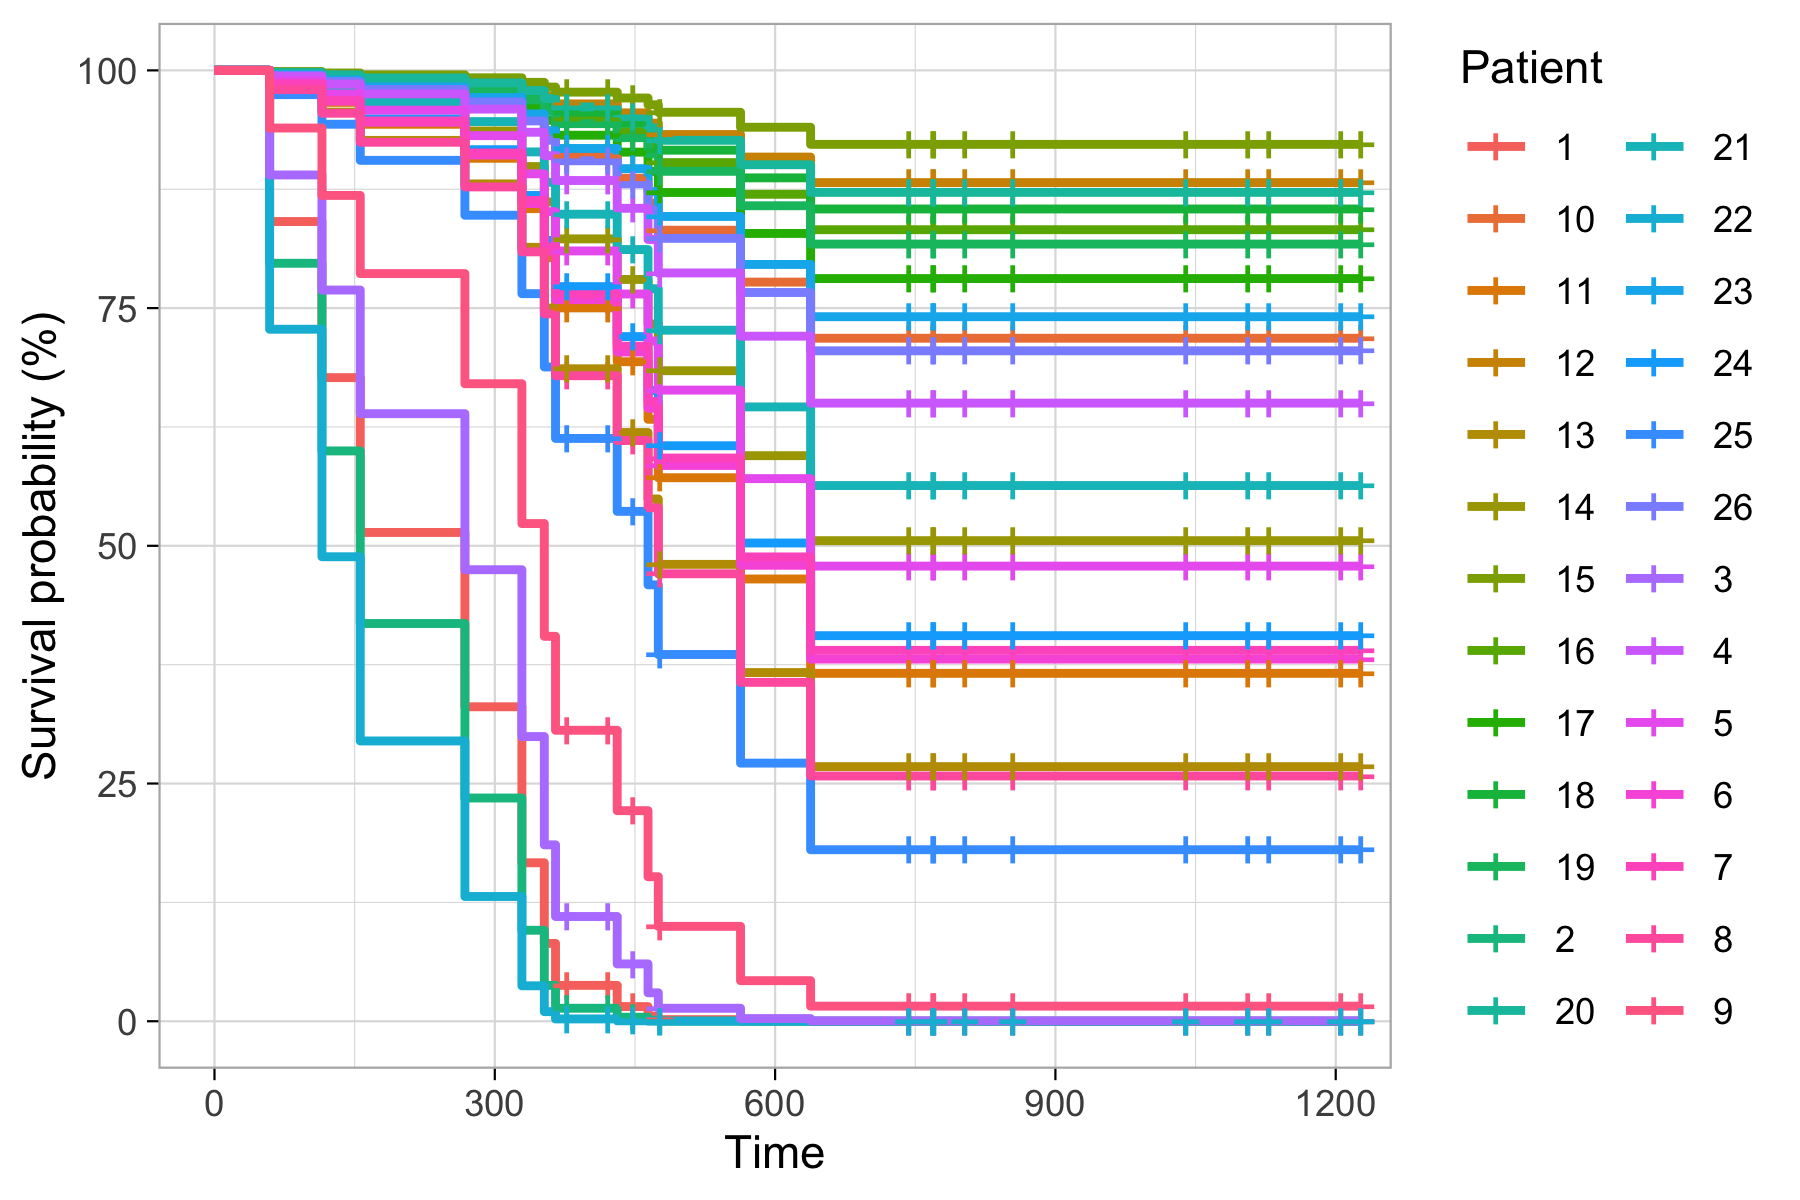
\includegraphics[width=0.9\textwidth]{img/ovarian-survplot-bypatient.png}\\
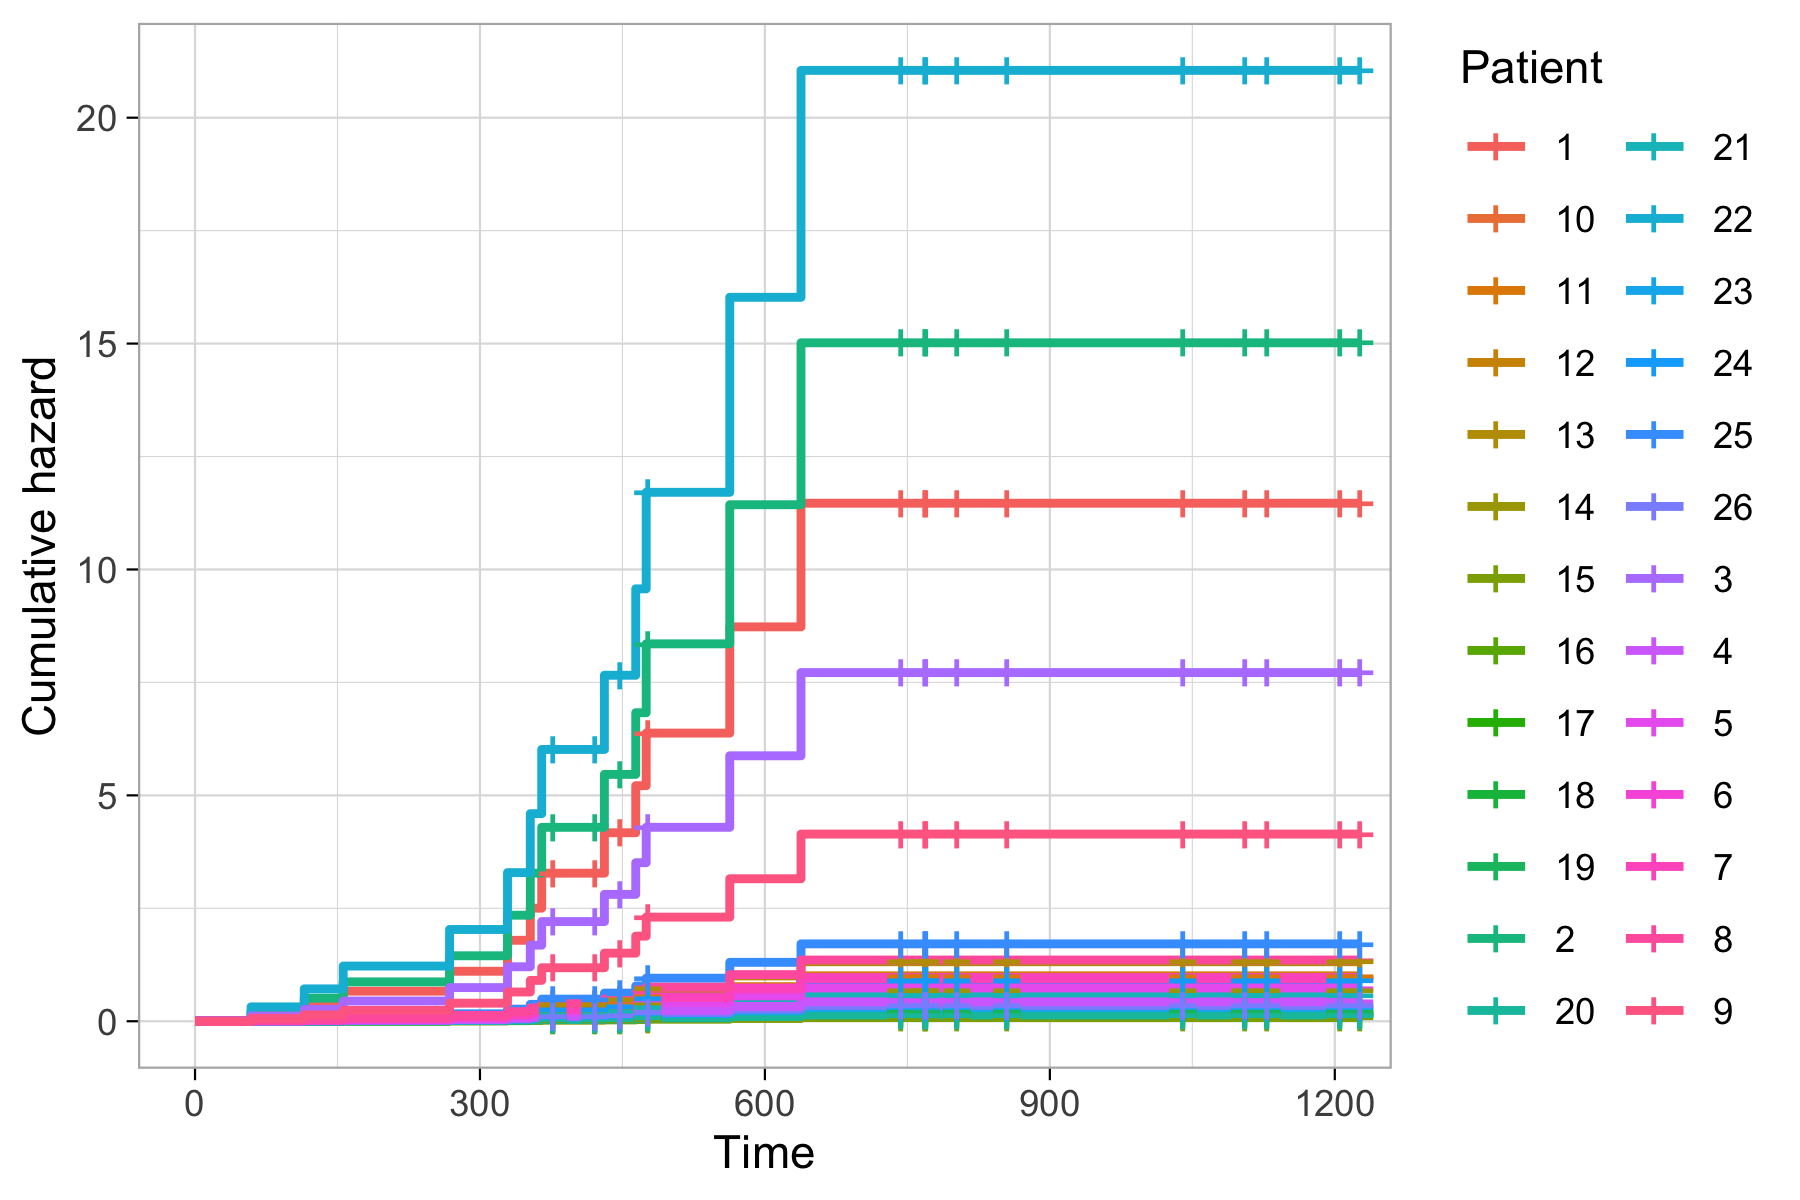
\includegraphics[width=0.9\textwidth]{img/ovarian-cumhaz-bypatient.png}
\end{center}

\newpage

\begin{question}{}
Which patients have the lowest and highest risk scores? Where do they appear on the patient-level survival and cumulative hazard graphs?
\end{question}

%%%%%%%%%%%%%%%%%%%%%%%%%%%%%%%%%%%%%%%%%%%%%%%%%%%%%%%%%%%%%%%%%%%%%%%%%%%%%%%%%%

\section{Testing the Proportional Hazards Assumption}

The Cox model makes three important assumptions:
\begin{enumerate}
\item \emph{Common baseline hazard.} At any time, $t$, all individuals experience the same baseline hazard, $\lambda_0(t)$. 
\item \emph{Proportional hazards.} The hazard for one individual is proportional to the hazard of any other individual.
\item \emph{Time-invariance.} The constant of proportionality between the hazards of any two individuals does not depend on time. 
\end{enumerate}
All of them are potentially problematic. In particular, it's hard to come up with situations in which the hazards for \emph{any} two individuals can reasonably be assumed to be proportional. Thus, it's important to check this assumption. 

There are whole book chapters and papers devoted to model diagnostics for the Cox model. I will present a couple of common methods here and leave the others to the course website. 

\subsection{Schoenfeld Residuals}

In Section~\ref{section:coxfit}, we saw how the Cox model was fit using maximization of the partial likelihood. The quantity
$$ \frac{\exp(\beta^Tx^{(i)})}{\sum_{l \in R(t_i)} \exp( \beta^Tx^{(l)})} $$ 
was important because it gave us the probability, according to the model, that the person observed to experience the event at time $t_i$ would experience it, given all the people in the risk set just prior to time $t_i$. The \textbf{Schoenfeld residual} capitalizes on this idea.

\begin{quote}
\textbf{Schoenfeld residual:} The covariate value $x_j^{(i)}$ for the person ($i$) who actually experienced the event at time $t_i$, minus the expected value of the covariate for the risk set at $t_i$. Or:
$$ \text{residual} = x_j^{(i)} - \sum_{l \in R(t_i)} x_j^{(l)} \frac{\exp(\beta^Tx^{(l)})}{\sum_{m \in R(t_i)} \exp( \beta^Tx^{(m)})} $$
\end{quote}

There is one Schoenfeld residual for each combination of observed event and covariate. Typically, they will be plotted against time to assess if there is a trend. The test for trend comes from a simple linear regression model of the residuals against time, conducted separately for each covariate. 

\begin{center}
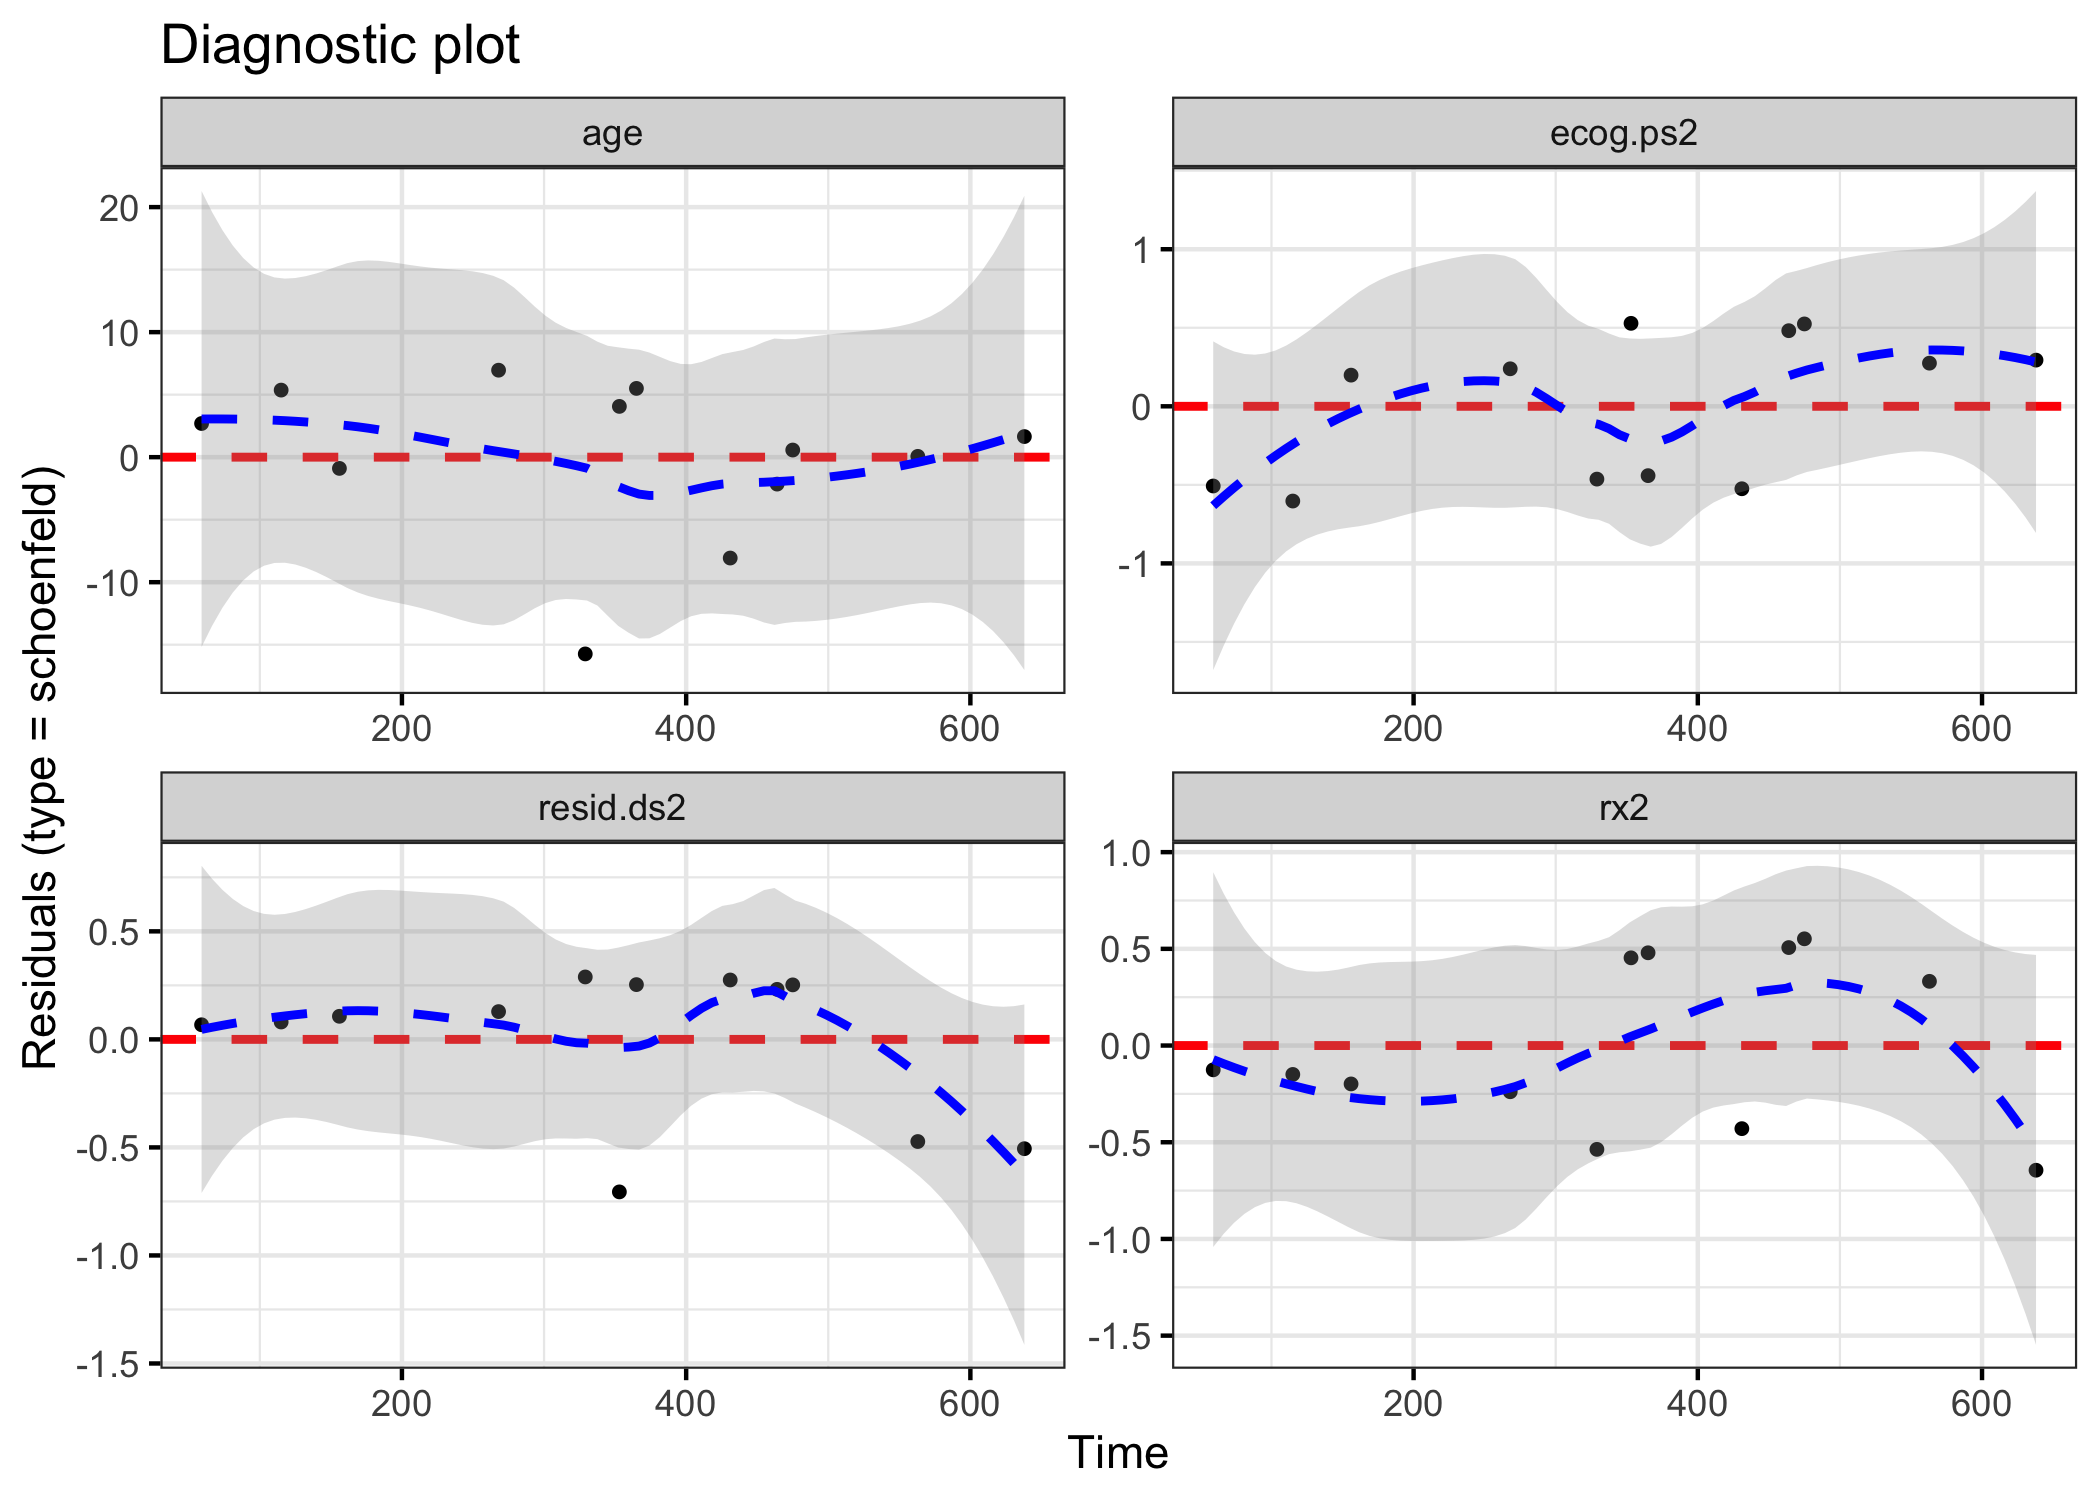
\includegraphics[width=0.9\textwidth]{img/ovarian-cox-diagnostics-schoenfeld.png}
\end{center}

\begin{question}{}
How would you conduct the test for trend for each covariate using a simple linear regression model?
\end{question}

\begin{question}{}
Try calculating the Schoenfeld residual for a single covariate and failure time (your choice). All of the information you need is in the table below. The \texttt{risk} column is the same as in the previous table. It is $\exp{(\beta^Tx)}$. 
{\small
\begin{center}
\begin{tabular}{rrrrrrrr}
  \hline
 & futime & fustat & age & resid.ds & ecog.ps & rx & risk \\ 
  \hline
1 & 59 & 1 & 72.33 & 2 & 1 & 1 & 14.43 \\ 
  2 & 115 & 1 & 74.49 & 2 & 1 & 1 & 18.90 \\ 
  3 & 156 & 1 & 66.47 & 2 & 2 & 1 & 9.71 \\ 
  22 & 268 & 1 & 74.50 & 2 & 2 & 1 & 26.49 \\ 
  23 & 329 & 1 & 43.14 & 2 & 1 & 1 & 0.38 \\ 
  24 & 353 & 1 & 63.22 & 1 & 2 & 2 & 1.14 \\ 
  25 & 365 & 1 & 64.42 & 2 & 1 & 2 & 2.16 \\ 
  26 & 377 & 0 & 58.31 & 1 & 1 & 2 & 0.44 \\ 
  4 & 421 & 0 & 53.36 & 2 & 1 & 2 & 0.54 \\ 
  5 & 431 & 1 & 50.34 & 2 & 1 & 1 & 0.93 \\ 
  6 & 448 & 0 & 56.43 & 1 & 2 & 1 & 1.21 \\ 
  7 & 464 & 1 & 56.94 & 2 & 2 & 2 & 1.18 \\ 
  8 & 475 & 1 & 59.85 & 2 & 2 & 2 & 1.71 \\ 
  9 & 477 & 0 & 64.18 & 2 & 1 & 1 & 5.21 \\ 
  10 & 563 & 1 & 55.18 & 1 & 2 & 2 & 0.42 \\ 
  11 & 638 & 1 & 56.76 & 1 & 2 & 1 & 1.27 \\ 
  12 & 744 & 0 & 50.11 & 1 & 1 & 2 & 0.16 \\ 
  13 & 769 & 0 & 59.63 & 2 & 2 & 2 & 1.66 \\ 
  14 & 770 & 0 & 57.05 & 2 & 1 & 2 & 0.86 \\ 
  15 & 803 & 0 & 39.27 & 1 & 1 & 1 & 0.10 \\ 
  16 & 855 & 0 & 43.12 & 1 & 2 & 1 & 0.23 \\ 
  17 & 1040 & 0 & 38.89 & 2 & 2 & 1 & 0.31 \\ 
  18 & 1106 & 0 & 44.60 & 1 & 1 & 1 & 0.20 \\ 
  19 & 1129 & 0 & 53.91 & 1 & 1 & 2 & 0.25 \\ 
  20 & 1206 & 0 & 44.21 & 2 & 1 & 2 & 0.17 \\ 
  21 & 1227 & 0 & 59.59 & 1 & 2 & 2 & 0.72 \\ 
   \hline
\end{tabular}
\end{center}
}
\end{question}

\begin{question}{}
The R function \texttt{cox.zph} performs the test of trend for all predictors as well as a global test of trend using ANOVA (don't worry, we'll get to this later). Here is the output for this model:
\begin{center}
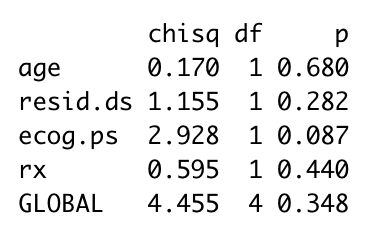
\includegraphics[width=0.4\textwidth]{img/ovarian-coxzph.png}
\end{center}
For which predictors is there a potentially worrying association between the Schoenfeld residuals and time?
\end{question}

\subsection{What to do if Violations are Found}

Interpretation of the Cox model is relatively insensitive to deviations from proportionality, especially for large sample sizes. However, if nonproportionality is a huge issue for one or more predictors, there are a few strategies to deal with it.

\begin{enumerate}
\item \emph{Stratify.} One can stratify the model by different levels of the problematic predictor(s), essentially building separate models for the other covariates at each different level of the problematic predictor(s). This only works for predictors that have discrete levels, however; otherwise, one would need to discretize. A potential downside is that stratification eliminates the model's ability to quantify the effect of the stratification variable(s).
\item \emph{Partition the time axis.} Sometimes proportionality holds for the first part of the time axis but falls apart at the end. In that case, one can analyze the data from the first part of the study separately. The disadvantage, of course, is that one must throw out information from later parts of the study.
\item \emph{Add a nonlinear effect term.} Continuous covariates with nonlinear effects on the outcome may lead to nonproportional hazards. Including transformations of these covariates may help to alleviate the nonproportional hazards. 
\end{enumerate}

